% -----------------------------------------------
% Vlastní text práce (kapitoly práce)
% -----------------------------------------------

% -----------------------------------------------
\chapter{Gamma rays detection}
% -----------------------------------------------


% -----------------------------------------------
\section{Properties and parameters of detectors}
% -----------------------------------------------
There 
The Mössbauer spectrometer setups on KEF are usually by gaseous or scintillation detectors.


\subsection{Gaseous detectors}
The gas detectors are usually tubes with electrodes with applied voltage around filled with a special gas mixture. According to the voltage, the gaseous detector can be operated in 3 regimes - proportional , or as a geiger counter. The second mode offers amplification. The advantage of gaseous detectors is that they offer good energy resolution.

\begin{figure}[H]
 \centering
 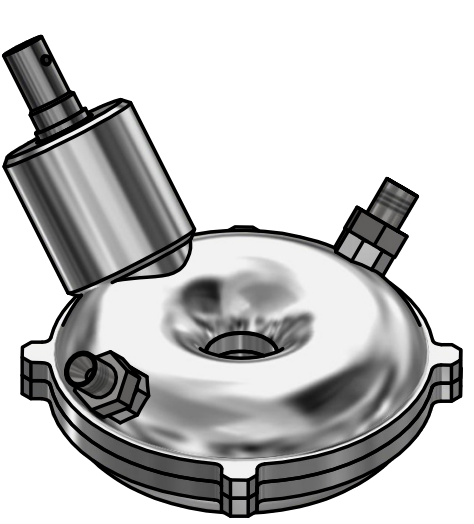
\includegraphics[scale=0.55, angle = 0]{./pictures/GASdet.png}
 \caption{Toroidal proportional gas flow counter used in MS spectrometer. \cite{Optimized}.}
 \label{toroid}
 
\end{figure}


\subsection{Scintillation detectors}
By scintillation detector is usually meant a scintillation crystal coupled with a photomultiplier tube (PMT). The first conversion happens inside scintillation crystal, where the incoming particle generates number of photons linearly dependent on its energy. These photons are captured by PMT's photo-cathode, where are they converted into electrons, and then multiplied on PMT's dynodes. This amplification requires high voltages around $1000 - 2000$ V.
\par
The PMT's have The internal amplification inside PMT can be around $10^6$. However, the energy resolution is not 
\par
The gamma spectra obtained this way usually have distorted wide peaks, which negatively affects Mössbauer spectrometry. The PMTs also cannot be employed in magnetic fields. 


\subsection{Detectors based on semiconductors}
The one problem with semiconductor detector is that there is no internal amplification, so the signals coming out of the detectors have to be amplified by electronics.
\par
The semiconductors are small and compact. They also don't require high voltage sources and heavy pressure cylinders. These facts can of making more compact Mössbauer spectrometers. The Mössbauer spectrometer MIMOS II \cite{•} based on 4 Si PIN diodes was a part a its mission to mars. 




% %%%%%%%%%%%%%%%%%%%%%%%% End of file %%%%%%%%%%%%%%%%%%%%%%%%